\chapter{Ferromagnetism}

    \section{Very weak itinerant ferromagnetism}
       
        Given the lowest-order finite-temperature correction to the Pauli susceptibility $\chi^{(0)}$ whose expression is
        \be
            \frac{\chi^{(0)}}{2\mu_\text{B}^2}\simeq \rho(\varepsilon_\text{F})+\frac{\pi^2}{12}\left[\rho''(\varepsilon_\text{F})-2\frac{\rho'^2(\varepsilon_\text{F})}{\rho(\varepsilon_\text{F})}\right]\,\left(k_\text{B}T\right)^2\, \label{eq:corPauli}
        \ee
        and using the generalized Stoner criterion one is able to derive the Curie temperature. One simply has to plug \eqref{eq:corPauli} into \eqref{eq:stoner} to get
        \be
            \frac{\pi^2k_\text{B}^2}{6}T_\text{C}^2=\frac{U\rho(\varepsilon_\text{F})-1}{\left[\frac{\rho'(\varepsilon_\text{F})}{\rho(\varepsilon_\text{F})}\right]^2-\frac{\rho''(\varepsilon_\text{F})}{\rho(\varepsilon_\text{F})}}\,
        \ee
   
        To develop the temperature dependence of the order parameter, one assumes
        \be
            \rho(\varepsilon)=\rho_0-a\varepsilon^2 \quad \text{with} \quad a>0\,
        \ee
        and one also assumes that the band is half-filled. One can then derive the temperature dependence of the order parameter. For this, one can minimize the free energy $\mc F=\mc E(T)-T\mc S$. The energy in the Stoner model is given by the following
        \be
            \mc E=\sum_\sigma \int_{-\infty}^{+\infty}\dd \varepsilon\ \varepsilon\rho(\varepsilon)f_\sigma(\varepsilon)+U(n^2-m^2)-g\mu_\text{B}Hm
        \ee
        where $f_\sigma$ is the Fermi distribution with the chemical potential $\mu_\sigma$ which satisfies
        \be
            \int_{-\infty}^{+\infty}\dd \varepsilon\ \rho(\varepsilon)f_\sigma(\varepsilon) = n+\eta(\sigma)m\,
            \label{eq:int-fermi}
        \ee
        with
        \be
            \eta(\sigma)=\begin{cases}
        1 & \text{ if } \sigma=\,\uparrow \\ 
        -1 & \text{ if } \sigma=\,\downarrow
        \end{cases}\,
        \ee
        The term $-T\mc S$ can be obtained considering the basic assumption of the Stoner theory that the entropy arises solely from the \electron-hole excitations, in other terms the entropy of band \electron. Using the following relation between the specific heat $C_V$ and the entropy
        \be
            C_V=T\left(\frac{\partial\mc S}{\partial T}\right)\,
        \ee
        and the usual expression of the low-temperature specific heat of the spin-$\uparrow$ and spin-$\downarrow$ bands, one can obtain
        \be
            -T\mc S=-\frac{(\pi k_\text{B}T)^2}{3}\sum_\sigma\rho(\mu_{\sigma,0})\,
        \ee
        with $\mu_{\sigma,0}=\mu_\sigma(T=0)$. Therefore one eventually has
        \be \begin{split}
            \mc F&=\sum_\sigma \int_{-\infty}^{+\infty} \dd \varepsilon\ \varepsilon\rho(\varepsilon)f_\sigma(\varepsilon)\,+U(n^2-m^2)\\ &-g\mu_\text{B}Hm-\frac{(\pi k_\text{B}T)^2}{3}\sum_\sigma\rho(\mu_{\sigma,0})\,
        \end{split}
        \ee
        One can see that $\mc F$ depends on $m$ both explicitly and via $\mu_\sigma$. One can take the derivative of both sides of \eqref{eq:int-fermi} with respect to $m$ and get, using both
        \be
            \frac{\partial f_\sigma}{\partial \mu_\sigma}=-\frac{\partial f_\sigma}{\partial\varepsilon}
        \ee
        and the Sommerfeld expansion and one should arrive at
        \be
            \frac{\partial\mu_\sigma}{\partial m}=\eta(\sigma) \left[\rho(\mu_{\sigma,0})-\frac{(\pi k_\text{B}T)^2}{3}\left(\frac{\rho'^2(\mu_{\sigma,0})}{\rho(\mu_{\sigma,0}}-\rho''(\mu_{\sigma,0})\right)\right]^{-1}\,
        \ee
        One can minimize $\mc F$ with respect to $m$ proceeding analogously to the derivation of the generalized Stoner criterion; and to order $T^2$, one finds the extremum condition to be
        \be
            (\mu_{\uparrow 0}-\mu_{\downarrow 0})-\frac{(\pi k_\text{B}T)^2}{6}\left[\frac{\rho'(\mu_{\uparrow 0})}{\rho(\mu_{\uparrow 0})}-\frac{\rho'(\mu_{\downarrow 0})}{\rho(\mu_{\downarrow 0})}\right]=2Um+g\mu_\text{B}H\,
        \ee
        The first assumption leads to
        \be
        \begin{split}
            \rho(\mu_{\uparrow 0}) &= \rho(\mu_{\downarrow 0})\simeq \rho_0-a\frac{m^2}{\rho_0^2} \\ \qq{and} \quad \rho'(\mu_{\uparrow 0}) &= -\rho'(\mu_{\downarrow 0})\simeq -\frac{2am}{\rho_0}\,
        \end{split}
        \ee
        First consider the case $H=0$. The spontaneous magnetization satisfies
        \be
            \frac{1}{\rho_0}\left[1+\frac{am^2}{\rho_0^3}\right])+\frac{(\pi     k_\text{B}T)^2}{3}\frac{a}{\rho_0^2}=U\,
        \ee
        At $T=0$, this yields
        \be
            m^2(0)=[U\rho_0-1]\frac{\rho_0^3}{a}\,
        \ee
        and requiring $m=0$ for $T=T_\text{C}$ gives
        \be
            \frac{\pi^2k_\text{B}^2}{3}T_\text{C}^2=(U\rho_0-1)\frac{\rho_0}{a}\,
        \ee
        Combining those two equations with the previous one, one obtains one of the most famous results of the Stoner model
        \be
            \frac{m^2(T)}{m^2(0)}=1-\left(\frac{T}{T_\text{C}}\right)^2\,
        \ee
        Eventually, allowing for the presence of $H\neq 0$, one can get the Edwards-Wohlfarth equation
        \be
            \frac{m^2(T,H)}{m^2(0,0)}=2\Tilde{\chi}\frac{H}{m(T,H)}+1-\left(\frac{T}{T_\text{C}}\right)^2\,
        \ee
        where
        \be
            \Tilde{\chi}=\frac{\rho_0g\mu_\text{B}}{U\rho_0-1}\,
        \ee
        
        One can use the previous result to derive the paramagnetic susceptibility. In a weak external field, one can omit the $m^2$ term to obtain
        \be
            \chi(T)=\frac{m(T,H)}{H}=\frac{2\Tilde{\chi}}{\left(\frac{T}{T_\text{C}}\right)^2-1}\,
        \ee

    \section{Lieb's Ferrimagnetism}
    
        In this second part one discusses a result stated by Elliot Lieb and Daniel Mattis about the ordering of energy levels of interacting spin systems. The original paper of Lieb and Mattis starts with the following the Hamiltonian
        \be
            \mc H =2\sum_{ij}J_{ij}\vb*{S}_i\cdot\vb*{S}_j
        \ee
        
        Consider a bipartite lattice which can be divided into two sublattices $A$ and $B$. Denote by $|A|$ and $|B|$ the number of sites in the sublattices and make one hypothesis: sublattices $A$ and $B$ are such that for all sites $i(A)$ on sublattice $A$ and $i(B)$ on sublattice $B$,
        \be
            J_{i(A)j(A)}\leq g^2\,,\quad J_{i(B)j(B)}\leq g^2\quad\text{and}\quad J_{i(A)j(B)}\geq g^2\,
            \label{eq:LiebConditions}
        \ee
        where $g^2$ is a positive constant. There are two cases
        \begin{itemize}
            \item there is at least one way to decompose the lattice into two sublattices that verify the above conditions \eqref{eq:LiebConditions}: one shall show that the system is either ferrimagnetic or antiferromagnetic.
            \item there is none, one cannot decompose the lattice in such a way that fulfills the conditions: then the system is not necessarily ferromagnetic and only explicit solutions can determine this.
        \end{itemize}
        One knows that the intrisic spin of an \electron is $1/2$ but to keep some generality, let the intrinsic spin be $S_i$. Define the total spins $S_A$ and $S_B$ on $A$ and $B$ sublattices as
        \be
            S_A = \sum_{i(A)}S_{i(A)}\quad \text{and} \quad S_B = \sum_{i(B)}S_{i(B)}\,
        \ee
        Eventually, we define
        \be
            \mc S = |S_A-S_B|\,
        \ee
        Then, the Lieb-Mattis ferrimagnetism theorem states that the ground state of $\mc H$ belongs at most to total spin $S_\text{tot}=\mc S$ and that for all $S_\text{tot}\geq\mc S$, one has
        \be
            E(S_\text{tot}+1)>E(S_\text{tot})\,
        \ee
            
        One shall restrict the discussion to the special case $g^2=0$ until the end of the proof.
                
        To sketch the proof first, recall that with the help of the total spin operator $S$ we can construct two operators that commute with the Hamiltonian, namely $\vb*{S}^2$ which possesses eigenvalues $S(S+1)$, and $S_z$ which possesses eigenvalues $M$. From the general theory of angular momentum, $-S\leq M\leq S$.

        It is then pretty obvious that every energy eigenvalue have a corresponding eigenstate in the $M=0$ subspace of eigenstates; every energy level except those belonging to $S=0$ have a corresponding eigenstate in the $M=1$ subpsace; every energy level except those belonging to $S=0$ and $S=1$ has a corresponding eigenstate in the $M=2$ subspace, and so on and so forth. Hence it follows that the inequality will be proved if one manages to show that the lowest energy in a given $M$ subspace belongs to $S=M$, since spin $S+1$ also has a corresponding eigenstate in this precise subspace. Therefore one would indeed have $E(S)<E(S+1)$.\\

        To detail the proof now, consider a $M$ subspace and choose the basis set formed of all distinct eigenstates of the spin values $S_i$ compatible with eigenvalues $M$. Denote each configuration in the set by $\ket{\phi_\alpha}$, where $\alpha$ is an index which runs over all members of the set. One shall provide a more precise expression of $\ket{\phi_\alpha}$ later on but before that let perform the following canonical transformation on the Hamiltonian $\mc H$
        \be
            \left\{\begin{matrix}
        S_{i(A)}^x & \longrightarrow  & -S_{i(A)}^x\\ 
        S_{i(A)}^y & \longrightarrow & -S_{i(A)}^y\\ 
        S_{i(A)}^z & \longrightarrow & S_{i(A)}^z
        \end{matrix}\right.
        \ee
        but do not change the spins on the $B$-sublattice. One can check that under the action of this canonical transformation the Hamiltonian splits in two parts
        \be
            \mc H \longrightarrow\mc H'=\mc H_0+\mc H_1\,
        \ee
        where $\mc H_0$ is the diagonal part
        \be
            \mc H_0=2\sum_iJ_{ij}S_i^zS_j^z\,
        \ee
        and $\mc H_1$ the off-diagonal part
        \be
            \mc H_1=-\sum_i\left(|J_{ij}|S_i^+S_j^-+S_i^-S_j^+\right)
        \ee
        with $S_i^+$ and $S_i^-$ the spin ladder operators
        \be
            S_i^\pm = S_i^x\pm\mathrm{i}S_i^y\,
        \ee
        For a given configuration $\alpha$, $S_i^z$ has eigenvalue $m_i$. One can then choose the following expression for our state
        \be
            \ket{\phi_\alpha}=C(S_1^+)^{S_1+m_1}(S_2^+)^{S_2+m_2}\dotsc(S_N^+)^{S_N+m_N}\ket{\chi}
        \ee
        where $\ket{\chi}$ is the state in which $m_i=-S_i$ such that
        \be \ket{\chi}=\ket{-S_1,-S_2,\dotsc,-S_N} \ee
        and $C$ is a positive normalization constant whose expression is of no use. Using this expression, it is obvious that if one defines $K_{\beta\alpha}$ as
        \be
            K_{\beta\alpha}=\bra{\phi_\beta}\mc H_1\ket{\phi_\alpha}
        \ee
        then $K_{\beta\alpha}\leq 0$, which allows to write $K_{\beta\alpha}=-|K_{\beta\alpha}|$.

        Denoting $\ket{\psi}$ the ground state in the $M$ subspace, which belongs to the ground-state energy $E_M$, one can write it as a linear combination of the configurations $\ket{\phi_\alpha}$ with amplitudes $c_\alpha$:
        \be
            \ket{\psi}=\sum_\alpha c_\alpha\ket{\phi_\alpha}\,.
        \ee
        For the diagonal part, introduce eigenvalues $E_\alpha$:
        \be
            \mc H_0\ket{\phi_\alpha}=E_\alpha\ket{\phi_\alpha}
        \ee
        and one can get
        \be
            -\sum_\beta |K_{\beta\alpha}|c_\beta+E_\alpha c_\alpha=E_M c_\alpha
            \label{eq:EAEM1}
        \ee
        Indeed, one has
        \begin{align}
            \mc H \ket{\psi}&=E_M\ket{\psi}\\
            \sum_\beta c_\beta\mc H \ket{\phi_\beta} &= \sum_\beta c_\beta E_M\ket{\phi_\beta} \\
            \bra{\phi_\alpha}\sum_\beta c_\beta\mc H \ket{\phi_\beta} &= \bra{\phi_\alpha}\sum_\beta c_\beta E_M\ket{\phi_\beta} \\
             \sum_\beta c_\beta\bra{\phi_\alpha}\mc H \ket{\phi_\beta}  &= \sum_\beta c_\beta E_M\bra{\phi_\alpha}\ket{\phi_\beta}
        \end{align}
        with $\braket{\phi_\alpha}{\phi_\beta}=\delta_{\alpha\beta}$ and
        \be
        \begin{split}
            \bra{\phi_\alpha}\mc H \ket{\phi_\beta} &=\bra{\phi_\alpha}\mc H_0\ket{\phi_\beta}+\bra{\phi_\alpha}\mc H _1\ket{\phi_\beta} \\ &=-|K_{\alpha\beta}|+E_\beta\delta_{\alpha\beta}=-|K_{\beta\alpha}|+E_\beta\delta_{\alpha\beta}
        \end{split}
        \ee
        one gets the expected result.

        Now, let attempt to construct another state in the $S=M$ subspace. Since that was just built the ground sate, if this trial state leads to the same energy it implies that the ground state is degenerate, otherwise one should obtain a larger energy. The state
        \be
            \ket{\psi'}=\sum_\alpha|c_\alpha|\ket{\phi_\alpha}
        \ee
        is a trial state with the energy $E_M$ and therefore it should verify the same equation derived before
        \be
            -\sum_\beta |K_{\beta\alpha}||c_\beta|+E_\alpha |c_\alpha|=E_M |c_\alpha|\,
            \label{eq:EAEM2}
        \ee
        Notice then that it is impossible for a single state $\ket{\phi_\alpha}$ to have an energy smaller than the ground state energy. Hence one should have
        \be
            E_\alpha-E_M>0
        \ee
        holding $\forall \alpha$. Which means that $|E_\alpha-E_M|=E_\alpha-E_M$. Using this, one can get two different expressions of $|(E_\alpha-E_M)c_\alpha|$. Indeed, according to \eqref{eq:EAEM1}
        \be
            |(E_\alpha-E_M)c_\alpha|=\left|\sum_\beta|K_{\beta\alpha}|c_\beta\right|\,
        \ee
        but according to \eqref{eq:EAEM2}
        \be
            |(E_\alpha-E_M)c_\alpha|=(E_\alpha-E_M)|c_\alpha|=\sum_\beta|K_{\beta\alpha}||c_\beta|\,
        \ee
        which eventually leads to
        \be
            \left|\sum_\beta|K_{\beta\alpha}|c_\beta\right|=\sum_\beta|K_{\beta\alpha}||c_\beta|\,
        \ee
        This is possible if and only if
        \be
            c_\beta \geq 0 \quad \forall \beta
        \ee
        In general one even has
        \be
            c_\beta > 0 \quad \forall \beta
        \ee
        To see this is true, one only has to suppose $c_\alpha=0$ for some $\alpha$. Then \eqref{eq:EAEM2} would yield
        \be
            \sum_\beta K_{\beta\alpha}|c_\beta|=0\,
        \ee
        and then one could establish that
        \be
            c_\alpha=0 \quad \forall \alpha
        \ee
        and this would leads to a situation where no wavefunction exists.

        There is actually an exception. If the Hamiltonian is broken into sets of non-interacting spins, that means that in some bonds the interactions are zero so one forms cluster of spins; it might also happen if the interaction is varied over a period of lattice spacing. The model as one designs it does not allow the latter.

        Therefore, in general, all amplitudes $c_\alpha$ are strictly positive and hence $E_M$ is non-degenerate. Indeed,  it is not possible to build a state orthogonal to $\ket{\psi}$ without violating the positivity criterion just established.

        Having proved the non-degeneracy on a general model, one can now consider only $A$-$B$ interactions and take $A$-$A$ and $B$-$B$ interactions to zero being this the most interesting case. One still have to prove the inequality. In other terms
        \be
            J_{i(A)j(A)}=J_{i(B)j(B)}=0\quad\text{and}\quad J_{i(A)j(B)}=J>0\,
        \ee
        The lowest energy belonging to each spin is given by $E(S)$ for $S\geq\mc S$, and the ground state belongs to $S=\mc S$. Indeed
        \be
            S=S_A+S_B \Longrightarrow S^2=S_A^2+S_B^2+2S_AS_B\,
        \ee
        hence eventually get
        \be
        \begin{split}
            2S_AS_B\ket{\psi} &=\left(S^2-S_A^2-S_B^2\right)\ket{\psi} \\ &=\left(S(S+1)-s_A(s_A+1)-s_B(s_B+1)\right)\ket{\psi}
        \end{split}
        \ee
        which gives the energy
        \be
            E(S)=J\left(S(S+1)-s_A(s_A+1)-s_B(s_B+1)\right)
        \ee
        This special Hamiltonian has an $S=M$ in each $M$ subspace such that $M\geq \mc S$. Therefore, so does $\mc H$. This completes the proof for $g^2=0$. The general proof, \emph{ie} for $g^2>0$, would consider $\mc H-g^2\vb*{S}^2$ instead of $\mc H$.

    \section{Nagaoka's ferromagnetism}

        One has seen that Ferromagnetism hardly arise in a proper way. Nagaoka's ferromagnetism is an important result for ferromagnetism to have a nice and solid basis. Indeed under some conditions Nagaoka's theorem states that a whole class of Hubbard model actually describes ferromagnetic state. Which means that the ground state is a fully polarized state. One will start by presenting a weak statement of the Nagaoka theorem and afterward, introducing mathematical results and discussing some interesting geometrical conditions, will reach the full statement. One will finally show the original proof of the theorem which is more complicated but yet very interesting mathematically.\\

        For the weak version, start with the usual Hubbard model
        \be
            \mc H = -\sum_{\sigma}\sum_{xy}t_{xy}c_{x\sigma}^{\dagger} c_{y\sigma} + \sum_{x}U_x n_{x\uparrow}n_{x\downarrow}
        \ee
        Assume that the hopping parameters satisfy $t_{xy} = t_{yx} > 0$. Also take the $U \rightarrow \infty$ limit and finally assume a perfect half-filling profile with one hole injected in a lattice site, so that $N_e = N-1$. Gathering all these conditions one can see that as a single hole living in a highly interacting spin cloud in the background. Nagaoka states that with this class of Hubbard model, among the ground states one correspond to the fully polarized state, thus ferromagnetic, with $S_{tot} = S_{max} = \frac{N_e}{2}$.\\

        First of all one needs to take into account the $U \rightarrow \infty$ limit and construct an effective Hamiltonian. Toward that purpose, consider the subspace of the whole Hilbert space which consist in all the states without any doubly occupied sites. Call it $\mathbb H_{N}^\text{hc}$. One can easily see that for any state $\ket{\psi} \in \mathbb H_{N}^\text{hc}$, $\mc H_\text{int}\ket{\psi} = 0$. Considering the orthogonal projection $P_\text{hc}$ onto $\mathbb H_{N}^\text{hc}$, one sees that the effective Hamiltonian could be taken as
        \be
            \mc H_\text{eff} = P_\text{hc}\mc H P_\text{hc}
        \ee
        which is an operator acting on $\mathbb H_{N}^\text{hc}$. Now need a basis to express this effective Hamiltonian and find its ground states. Build them taking into account that they have to depend on the position of the hole as well as the spin configuration of the whole lattice. Thus define
        \be
            \ket{\phi_{x\Tilde{\sigma}}} = c_{x\uparrow}\left(\prod_{y}c^{\dagger}_{y\Tilde{\sigma}_y'}\right)\ket{0} = c_{x\downarrow}\left(\prod_{y}c^{\dagger}_{y\Tilde{\sigma}_y''}\right)\ket{0}
        \ee
        One wants to examine the effect of $H_\text{eff}$ on this state. Start by applying $\sum_{\sigma}c^{\dagger}_{x\sigma}c_{z\sigma}$. Developing
        \be
        \begin{split}
            \sum_{\sigma}c^{\dagger}_{x\sigma}c_{z\sigma}\ket{\phi_{x\Tilde{\sigma}}} &= -c_{z\uparrow}\left(\prod_{y}c^{\dagger}_{y\Tilde{\sigma}_y'}\right)\ket{0} -c_{z\downarrow}\left(\prod_{y}c^{\dagger}_{y\Tilde{\sigma}_y'}\right)\ket{0}\\ &= -\ket{\phi_{z\Tilde{\sigma}_{z\rightarrow x}}}
        \end{split}
        \ee
        where $\Tilde{\sigma}_{z\rightarrow x}$ is the new spin configuration obtained by moving $\sigma_{z}$ to $x$. Using this result, end up with
        \be
            \bra{\phi_{y\Tilde{\tau}}}H_{eff}\ket{\phi_{x\Tilde{\sigma}}} = \left\{
            \begin{array}{ll}
                -t_{xy} & \text{if } \Tilde{\tau} = \Tilde{\sigma}_{y\rightarrow x} \\
                0 & \text{otherwise}
            \end{array}
        \right.
        \ee
        One is now able to construct a ground state with respect to this basis. Therefore
        \be
            \ket{\phi_\text{GS}} = \sum_{x}\sum_{\{\Tilde{\sigma}\}} \phi(x,\Tilde{\sigma})\ket{\phi_{x\Tilde{\sigma}}}
        \ee
        Out of convenience, write
        \be
            \xi_x^2 = \sum_{\{\Tilde{\sigma}\}} \phi^2(x,\Tilde{\sigma})
        \ee
        so that the corresponding normalized ferromagnetic state is
        \be
            \ket{\phi_\text{FM}} = \sum_{x}\xi_x\ket{\phi_{x(\uparrow)}}
        \ee
        where $(\uparrow)$ is the spin configuration with all spins up.
        Finally compare the energies of the so-built ground state and the ferromagnetic state
         \be
          \begin{aligned}
           \bra{\phi_\text{GS}} \mc H_\text{eff}\ket{\phi_\text{GS}} & = \sum_{xy}\sum_{\{\Tilde{\sigma}\}\{\Tilde{\tau}\}}\phi(y,\Tilde{\tau})\phi(x,\Tilde{\sigma})\bra{\phi_{y\Tilde{\tau}}}\mc H_\text{eff}\ket{\phi_{x\Tilde{\sigma}}} \\
             & = -\sum_{xy}t_{xy}\sum_{\{\Tilde{\sigma}\}}\phi(y,\Tilde{\sigma}_{y\rightarrow x})\phi(x,\Tilde{\sigma}) \\
             & \geq -\sum_{xy}t_{xy}\left[\sum_{\{\Tilde{\sigma}\}}\phi^2(y,\Tilde{\sigma}_{y\rightarrow x})\right]^{\frac{1}{2}}\left[\sum_{\{\Tilde{\sigma}\}}\phi^2(x,\Tilde{\sigma})\right]^{\frac{1}{2}} \\
             & = \bra{\phi_\text{FM}} \mc H_\text{eff}\ket{\phi_\text{FM}}
          \end{aligned}
        \ee
        Thus $\ket{\phi_\text{FM}}$ is also a ground state.\\

        The extension of the Nagaoka theorem is mainly based of the Perron-Frobenius theorem, which one will state but not prove. The stronger statement enables to show that the FM state is actually the only ground state -- up to trivial degeneracy.


        Now, introduce the Perron-Frobenius theorem. Let $M$ be an $N\times N$ real and symmetric matrix with the following properties
        \begin{itemize}
            \item $M_{ij} < 0$ $\forall i,j$
            \item ll $i \neq j$ are connected by non-vanishing elements of $M$
        \end{itemize}
        Then the lowest eigenvalue of $M$ is non-degenerate.

        One can see that the Perron-Frobenius theorem can provide the fact that the ferromagnetic ground state is indeed the only ground state. From what is already derived, one knows that the effective Hamiltonian matrix elements are negative so one needs to add the connectivity notion to the Hubbard model in order to have the final class of model that predicts exact ferromagnetism.

        When it is said that every $i\neq j$ has to be connected via non-vanishing elements of the matrix $M$, it means that it exists a sequence $(i_1,i_2,\dotsc,i_K)$ with $i_1=1$ and $i_K=j$ such that $m_{i_k,i_{k+1}} \neq 0$.

        \begin{figure}[h!]
            \centering
            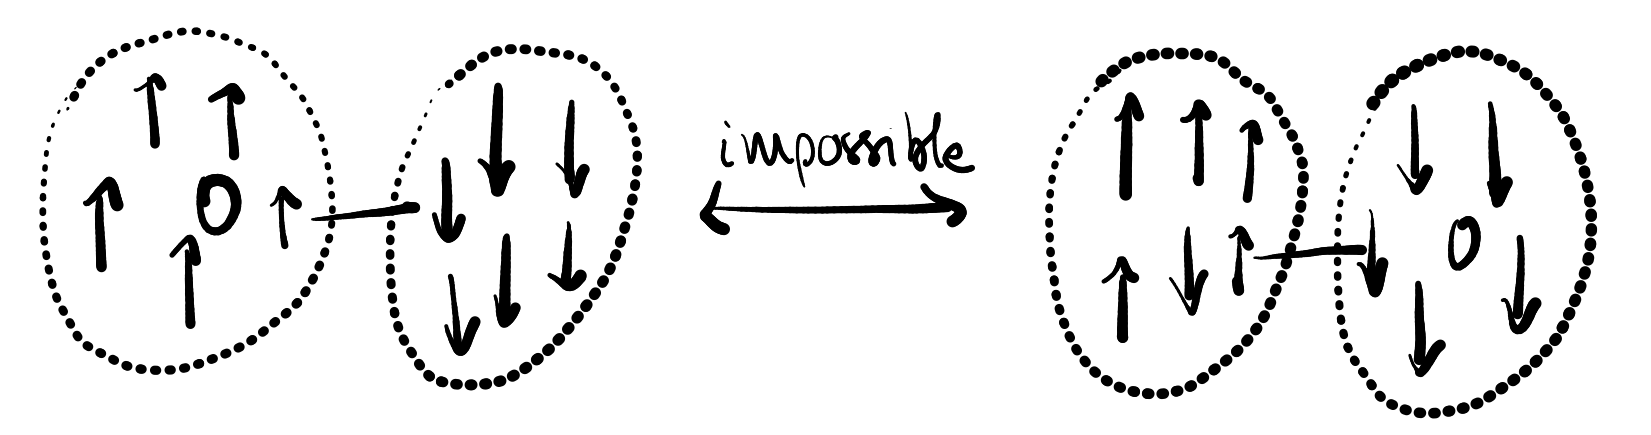
\includegraphics[scale=0.2]{graphs/nonBiconnected.png}
            \caption{Non-biconnected lattice}
            \label{fig:nonBiconnected}
        \end{figure}

        In the sense of Nagaoka it means that the matrix elements 
        \be \bra{\phi_{x\Tilde{\sigma}}}\mc H_\text{eff}\ket{\phi_{y\Tilde{\tau}}} \ee
        has to be connected in the sense of Perron-Frobenius. Since every basis vector contains the spin configuration of the lattice, one can have a more geometrical sense of the connectivity. Indeed one can say that a Hubbard model is connected if one can pass from one configuration to another by hoppings of the hole. As a matter of fact, in 1D, very few lattices are connected. However in 2D or higher dimension, apart from a couple of examples, all lattices are connected. \autoref{fig:nonBiconnected} and \autoref{fig:pentagon} are examples of 2D lattices that are clearly not connected.\\

        \begin{figure}[h!]
            \centering
            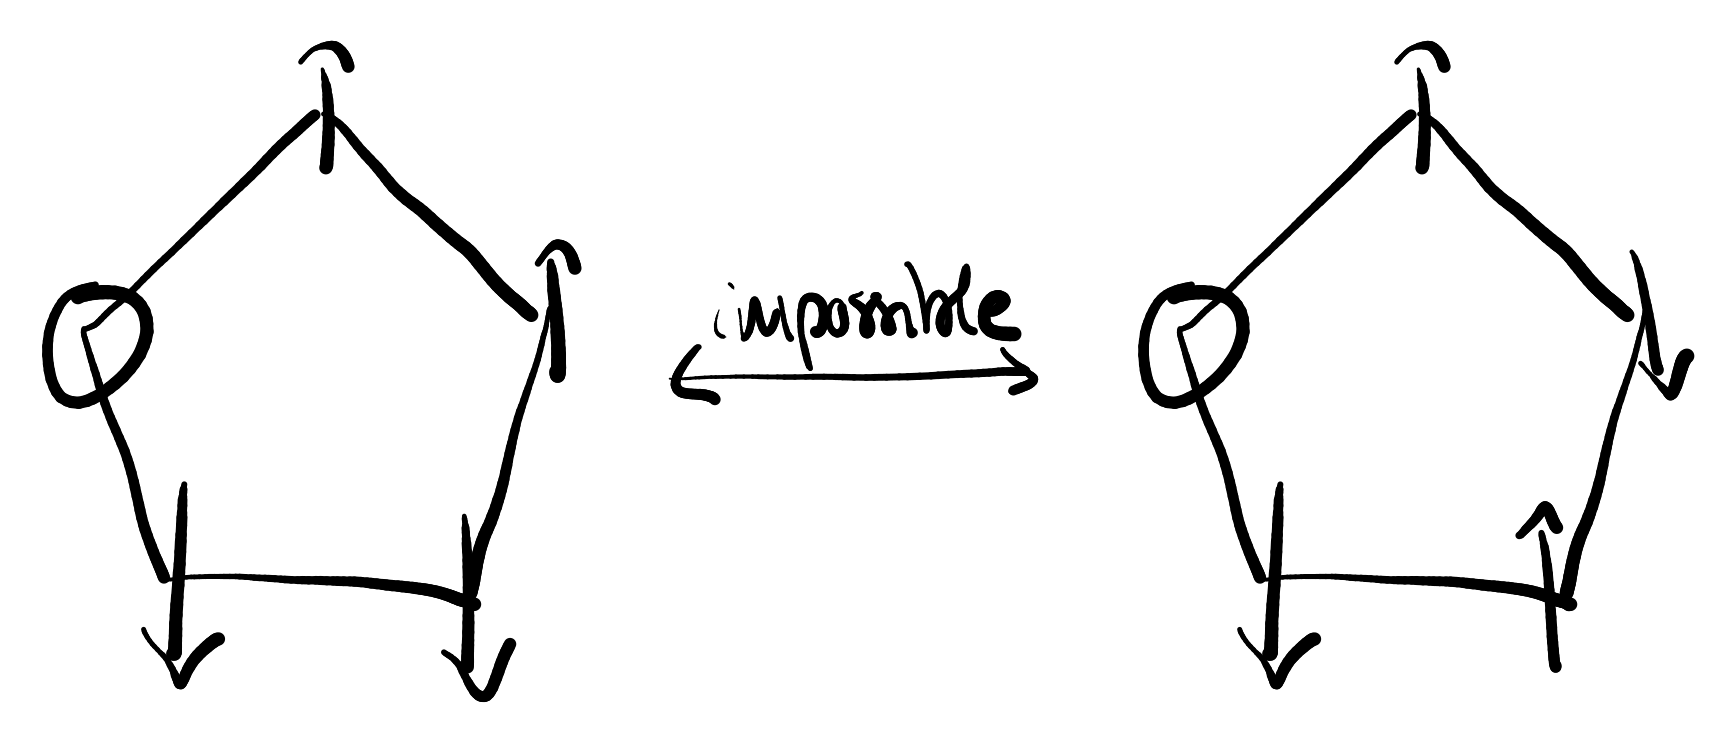
\includegraphics[scale=0.15]{graphs/pentagon.png}
            \caption{Pentagon lattice}
            \label{fig:pentagon}
        \end{figure}
     
        The following aims at giving the idea of this proof as it is certainly interesting but now obsolete since one has the previous really solid proof. First of all, Nagaoka uses the Hamiltonian
        \be
            \mc H = t\sum_{\langle ij \rangle}\sum_{\sigma}c_{i\sigma}^{\dagger}c_{j\sigma}
        \ee
        And show that the fully polarized state has $S=S_\text{max}$ and $E = -zt$, where $z$ is the number of nearest neighbors. The idea of the theorem proof will be to show that no energies are possible below $-zt$ and that no ground state with $S<S_\text{max}$ exists either.
        \newline
        Define the notion of superlattice which is the set $\{i_{\alpha_i} \}_{i,\alpha}$ for which each element corresponds to one site in one lattice configuration. Define a scalar product given by
        \be
        (j_{\beta_j}|i_{\alpha_i})_{\omega} = \bra{\psi_{j\beta_j}}\frac{1}{w-H}\ket{\psi_{i\alpha_i}}
        \ee
        where $\omega$ is any complex number. The poles of $(i_{\alpha_i}|i_{\alpha_i})_{\omega}$ define the eigenvalues of $\mc H$ that lie on the real axis. After some calculation one ends up with
        \be
        (i_{\alpha_i}|i_{\alpha_i})_{\omega}^{-1} = \omega[1-f(\omega)]
        \ee
        with             
        \be
        f(\omega) = \sum_{p=2}^{\infty}\frac{A_p}{z^p}\left( \frac{-zt}{\omega}\right)^p
        \ee
        After analyzing this series, one deduces that it is absolutely convergent for $\omega<-zt$. Thus for $\omega<-zt$, $(i_{\alpha_i}|i_{\alpha_i})_{\omega}$ is well defined and so has no pole. Hence, no energy below $-zt$ is allowed.

    \section{The ring-exchange mechanism}

        Now, one is going to focus one special type of lattice, from which will be deduced some properties of quasi-equivalent physical systems. 

        \begin{figure}[h!]
            \centering
            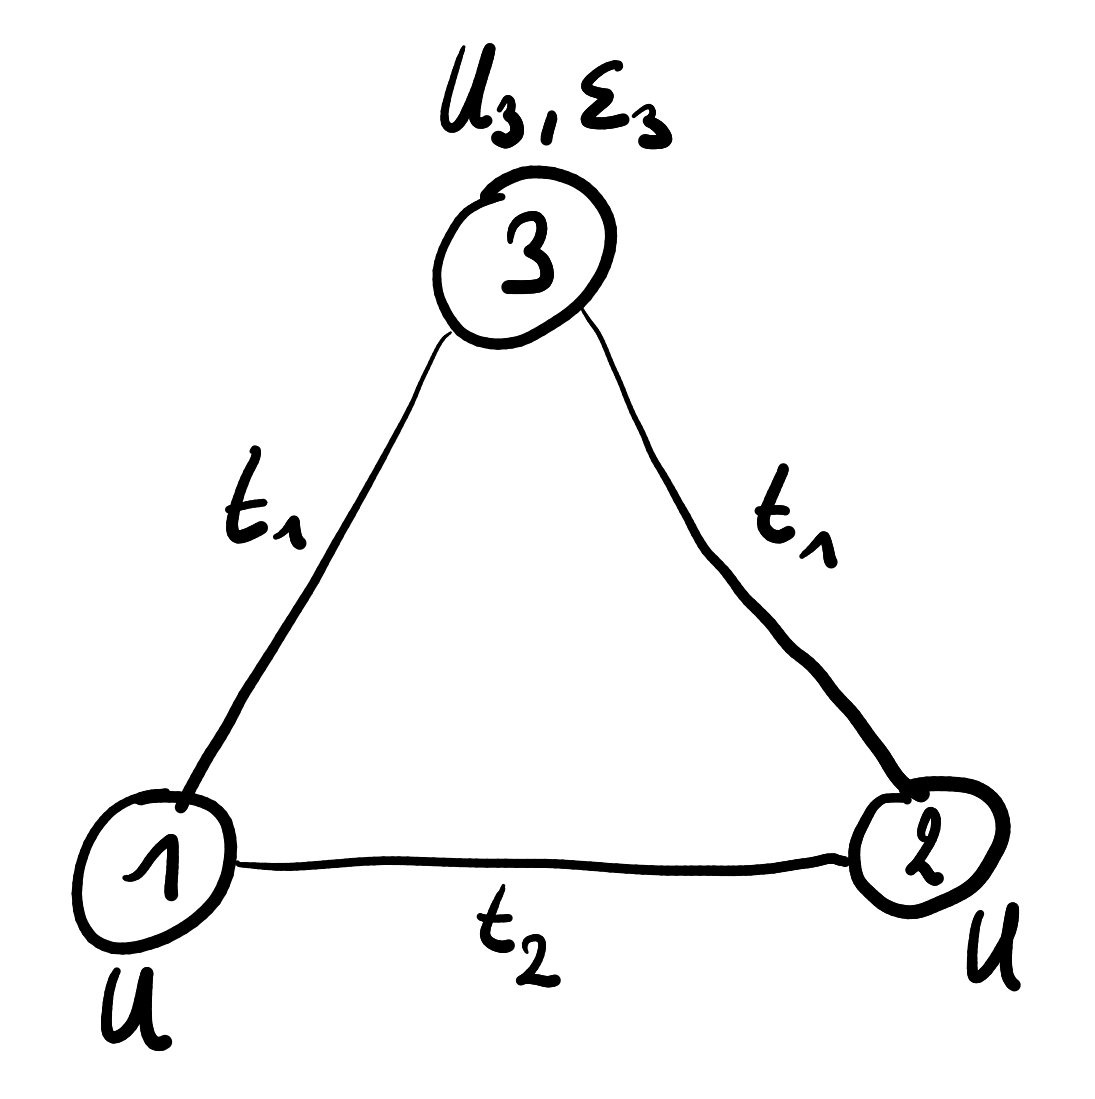
\includegraphics[scale=0.15]{graphs/threeSiteToy.png}
            \caption{Three-site toy model.}
            \label{fig:threeSiteToy}
        \end{figure}

        To the end, consider the 3-site toy model given in \autoref{fig:threeSiteToy}. Its Hubbard Hamiltonian can be easily written as
        \be \begin{split} \mc H_3 &=t_2 \sum_\sigma [c^\dagger_{1\sigma} c_{2\sigma} + c^\dagger_{2\sigma} c_{1\sigma}] + U\sum_{i=1,2} n_{i\uparrow} n_{i\downarrow} \\ &+ t_1 \sum_\sigma [c^\dagger_{1\sigma} c_{3\sigma} + c^\dagger_{2\sigma} c_{3\sigma} + c^\dagger_{3\sigma} c_{1\sigma} + c^\dagger_{3\sigma} c_{2\sigma}] \\ &+ U_3 n_{3\uparrow} n_{3\downarrow} + \varepsilon_3 \sum_\sigma n_{3\sigma} \end{split} \ee
        The system is considered to be ferromagnetic if its ground state is a triplet, while non-magnetic if it is a singlet. The interest of this three-site toy model is that, for a wide range of parameters, there is a triplet ground state and its ferromagnetism is quite the same as for the Tasaki's 1D chain model shown on \autoref{fig:tasaki1DChain}. 
        
         \begin{figure}[h!]
            \centering
            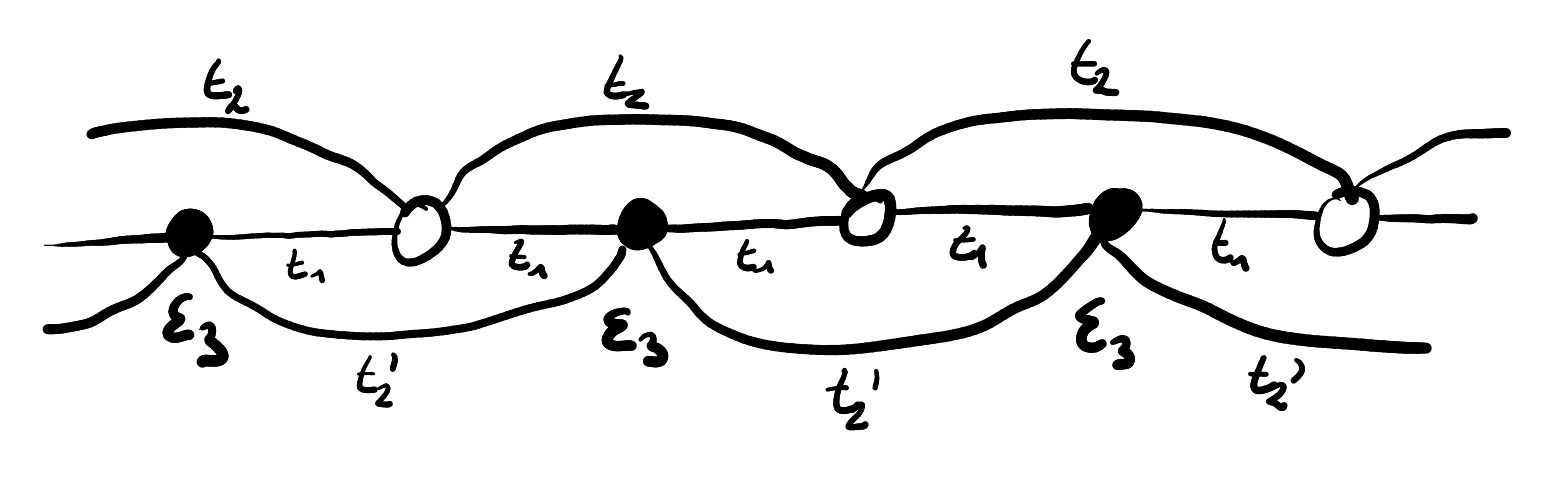
\includegraphics[scale=0.2]{graphs/tasaki1DChain.png}
            \caption{Tasaki's 1D chain.}
            \label{fig:tasaki1DChain}
        \end{figure}
        
        Starting with the case of 1\electron which shall be useful later, one can note that the system only has a symmetry with respect to the axis passing through site 3. From this and even without involving group representations theory, one observes that the antisymmetric state
        \be \ket{\psi_o} = \frac{1}{\sqrt{2}}[\ket 1 - \ket 2] \ee
        does not mix with $\ket 3$. Casting the states in their fermionic form
        \be \ket i = c^\dagger_{i\sigma} \ket 0 \ee
        labelling $\ket 0$ the vacuum, one finds the action of the Hamiltonian on $\ket{\psi_o}$ as
        \be \begin{split} \mc H_3 \sqrt 2 \ket{\psi_o} &= t_2 [c^\dagger_{2\sigma}c_{1\sigma}c^\dagger_{1\sigma} - c^\dagger_{1\sigma}c_{2\sigma}c^\dagger_{2\sigma}] \ket 0 \\ &+ t_1 [c^\dagger_{3\sigma}c_{1\sigma}c^\dagger_{1\sigma} - c^\dagger_{3\sigma}c_{2\sigma}c^\dagger_{2\sigma}] \ket 0 \\ &=  t_2 [c^\dagger_{2\sigma}(1-\cancel{c^\dagger_{1\sigma}c_{1\sigma}}) - c^\dagger_{1\sigma}(1-\cancel{c^\dagger_{2\sigma}c_{2\sigma}})] \ket 0 \\  &+ t_1 [c^\dagger_{3\sigma}(\cancel 1-\cancel{c^\dagger_{1\sigma}c_{1\sigma}}) - c^\dagger_{3\sigma}(\cancel 1-\cancel{c^\dagger_{2\sigma}c_{2\sigma}})] \ket 0  \\
        &= t_2 [\ket 2 - \ket 1] = -t_2 \sqrt 2 \ket{\psi_o} \end{split} \ee
        Hence denote $\lambda_0 = -t_2$ its eigenvalue. Performing the same computations for the symmetric state 
        \be \ket{\psi_e} = \frac{1}{\sqrt{2}}[\ket 1 + \ket 2] \ee
        that now mixes with $\ket 3$ as
        \be \begin{aligned} &\mc H_3 \ket{\psi_e} = t_2 \ket{\psi_e} + t_1 \sqrt 2 \ket 3 \\  &\mc H_3 \ket 3 = t_1 \sqrt 2 \ket{\psi_e} + \varepsilon_3 \ket 3 \end{aligned} \ee
        Diagonalizing $\mc H_3$ in the subspace spanned by $\{ \ket{\psi_o},\ket 3\}$ yields
        \be 0 = (t_2 - \lambda)(\varepsilon_3 - \lambda) - 2t_1^2 = \lambda^2 -\lambda(t_2 + \varepsilon_3) + t_2 \varepsilon_3 - 2t_1^2 \ee
        and then the eigenenergies for the triplet states
        \be \lambda_e ^\pm = \frac{t_2 + \varepsilon_3 \pm \sqrt{(t_2 - \varepsilon_3)^2+8t_1^2}}{2} \ee
        Note that one does not care about the sign of $t_1$ since appearing squared. Hence, fix $t_1>0$ which can be justified by changing the sign of $t_1$ being equivalent to the canonical transformation $c^\dagger_{3\sigma} \to - c^\dagger_{3\sigma}$, $c_{3\sigma} \to - c_{3\sigma}$.
        
        The case with 2\electron is more interesting. Begin with the system for which doubly-occupied sites are forbidden, that is $U=U_3=\infty$. Use the following notation in the $S^z=0$ subspace, \emph{eg}
        \be \ket{\uparrow\downarrow 0} = c^\dagger_{1\uparrow}c^\dagger_{2\downarrow} \ket 0 \ee
        There are 6 states in total. To find the ground states, it is useful to note that the exchange of 2 spins can be viewed as an exchange in a ring with the hole hopping through the sites as in \autoref{fig:ring}, since doubly-occupied sites are impossible.
        
        \begin{figure}[h!]
            \centering
            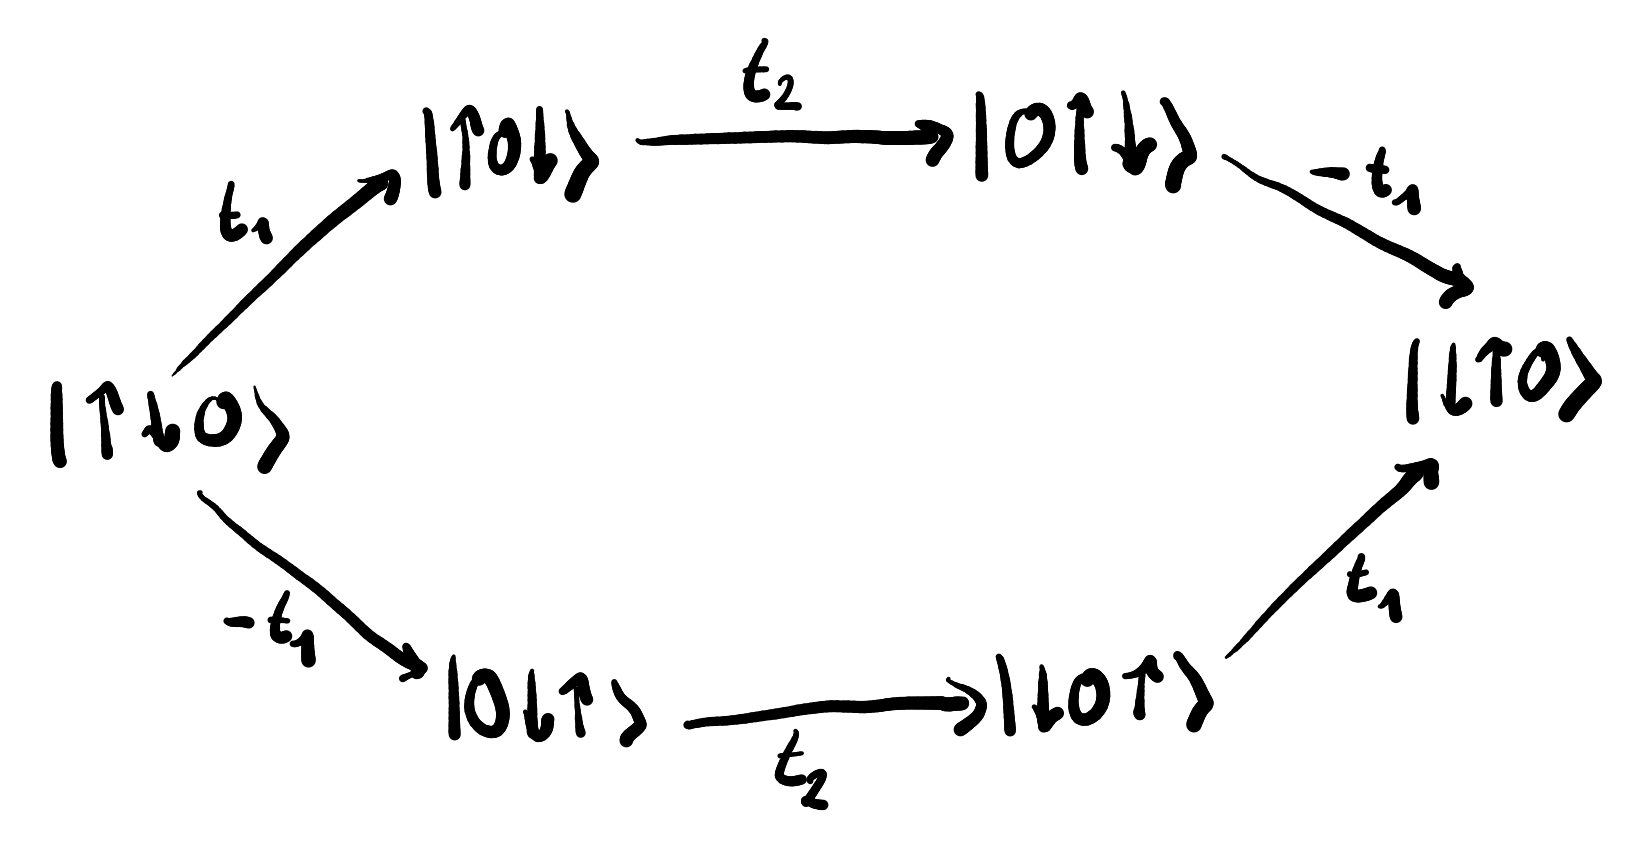
\includegraphics[scale=0.15]{graphs/ring.png}
            \caption{Ring exchange mechanism.}
            \label{fig:ring}
        \end{figure}
        
        It is important to note the sign of the matrix elements since they impose some constraints on the states possible. Using the argument, coming from the Perron-Frobenius theorem, that the sign between 2 states is the opposite of the one of the corresponding matrix element to lower the energy at each hopping process, one finds for $t_2<0$
        \be \ket{\psi_\text{GS}}_{t_2<0} = \underbrace{\frac{1}{\sqrt 2} [\ket{\uparrow\downarrow 0} - \ket{\downarrow \uparrow 0}]}_{\ket \alpha} + \underbrace{\frac{\alpha}{2}[\ket{0\downarrow\uparrow} - \ket{0\uparrow\downarrow} + \ket{\downarrow 0 \uparrow} - \ket{\uparrow 0 \downarrow}]}_{\alpha\ket \beta} \ee
        which is made of 3 singlets, thus is a singlet. For $t_2>0$
        \be \ket{\psi_\text{GS}}_{t_2>0} = \frac{1}{\sqrt 2} [\ket{\uparrow\downarrow 0} + \ket{\downarrow \uparrow 0}] + \frac{\beta}{2}[\ket{0\downarrow\uparrow} + \ket{0\uparrow\downarrow} - \ket{\downarrow 0 \uparrow} - \ket{\uparrow 0 \downarrow}] \ee
        and this is a triplet. Therefore, one found that the system is ferromagnetic when $U=\infty$ and $t_2>0$. It is important to note that for $U=0$, the ground state is a singlet, thus non-magnetic. This implies that there must exists a phase transition at a finite $U$.
        
        To find the phase boundary, one has to find the energies of the singlet and triplet states and compare them. For the triplet, spins must be parallel then one must take the 2 lowest-energy single \electron states, hence using the previously found eigenenergies
        \be \varepsilon_t = \lambda_o + \lambda_e^- =  \frac{\varepsilon_3 - t_2 - \sqrt{(t_2 - \varepsilon_3)^2+8t_1^2}}{2} \ee
        Then, for the singlet, find the action of $\mc H_3$ on the singlet pairs, introducing $\ket{\gamma_{12}} = \frac{1}{\sqrt 2} [c^\dagger_{1\uparrow} c^\dagger_{1\downarrow} + c^\dagger_{2\uparrow}c^\dagger_{2\downarrow}] \ket 0$ and $\ket{\gamma_3} = c^\dagger_{3\uparrow}c^\dagger_{3\downarrow} \ket 0$,
        \be \begin{split} &\mc H_3 \ket \alpha = t_1 \sqrt 2 \ket \beta + 2 t_2 \ket{\gamma_{12}} \\ &\mc H_3 \ket \beta = t_1 \sqrt 2 \ket \alpha + (t_2 + \varepsilon_3) \ket \beta + t_1 \sqrt 2 \ket{\gamma_{12}} + 2t_1 \ket{\gamma_3} \\ &\mc H_3 \ket{\gamma_{12}} = 2t_2 \ket \alpha + t_1 \sqrt 2 \ket \beta + U \ket{\gamma_{12}} \\ &\mc H_3 \ket{\gamma_3} = 2t_1 \ket \beta + (2\varepsilon_3 + U_3) \ket{\gamma_3} \end{split} \ee
        Again, using $U=U_3=\infty$, diagonalize in the subspace $\{\ket \alpha ,\ket \beta \}$ and find
        \be \varepsilon_s = \frac{\varepsilon_3 + t_2 - \sqrt{(t_2 + \varepsilon_3)^2+8t_1^2}}{2} \ee
        
        \begin{figure}[h!]
            \centering
            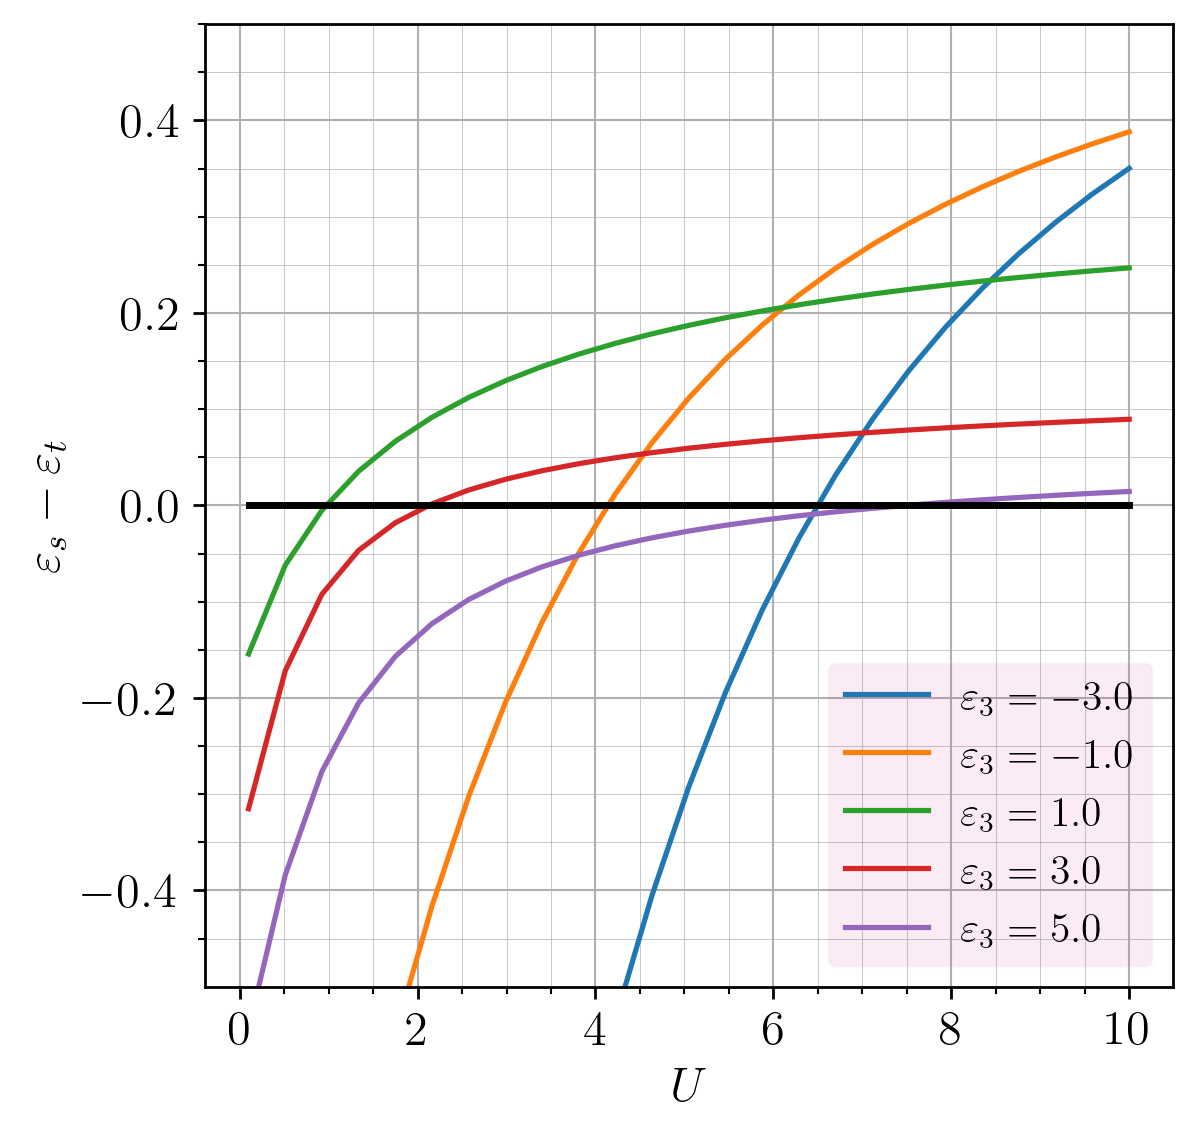
\includegraphics[scale=0.65]{graphs/diff.png}
            \caption{Energy difference $\varepsilon_s - \varepsilon_t$ for as a function of $U$ for different values of $\varepsilon_3$.}
            \label{fig:diff}
        \end{figure}

        It is possible although boring to check that $\varepsilon_t<\varepsilon_s$ for $t_2>0$, confirming the previous argument. For the full problem, numerical solution gives finite-$U$ transitions, appearing for smaller $U$ when $\varepsilon_3$ increases, as shown on \autoref{fig:diff}. However, $\varepsilon_3$ must stay negative, since when is becomes positive, increasing it seems to make the transition occur at a larger $U$, as shown on \autoref{fig:cross}. This indicates a dependence in the sign and value of $\varepsilon_3$ in the effective Hamiltonian.
        
        \begin{figure}[h!]
            \centering
            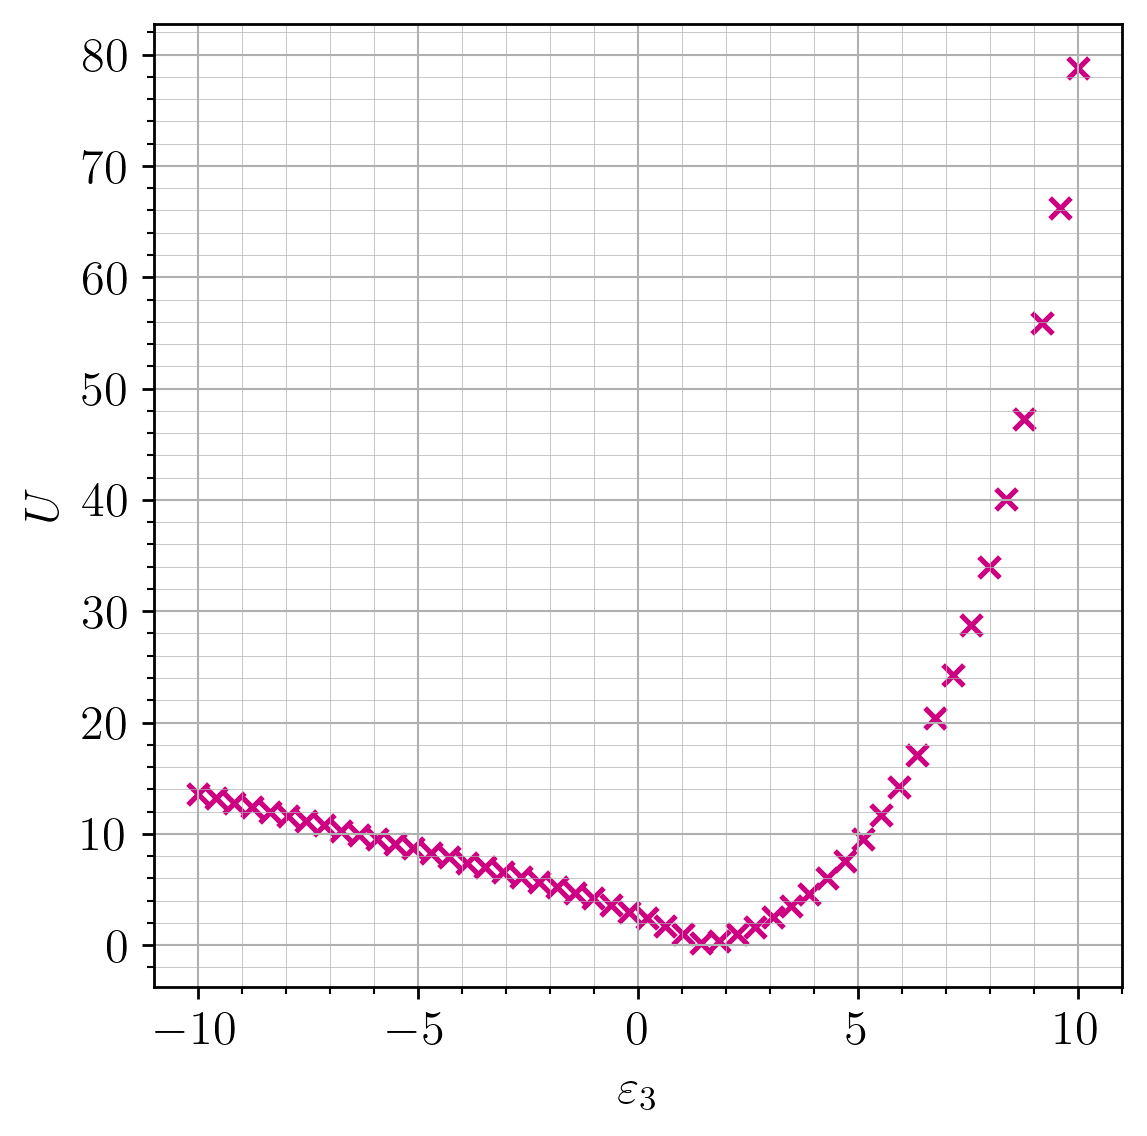
\includegraphics[scale=0.65]{graphs/cross.png}
            \caption{Values of $U$ for which the transition occurs as a function of $\varepsilon_3$.}
            \label{fig:cross}
        \end{figure}

        Now, consider the finite case $U>\varepsilon_3 \gg t_1, t_2$, $U_3 = \infty$. The eigenvalue problem can be solved in $\{\ket \alpha ,\ket \beta, \ket{\gamma_{12}} \}$, and expanding in $t_1,t_2$ gives the effective Hamiltonian
        \be \mc H_\text{eff} \simeq \underbrace{\left[\frac{4t_2^2}{U} -\frac{4t_2t_1^2}{\varepsilon_3^2}\right]}_{J} \vb*{S_1} \cdot \vb*{S_2} \ee
        with $J$ thus coupling constant being defined here as the difference $\varepsilon_t - \varepsilon_s$ up to high orders. The third order term is precisely the ring exchange presented above. And once again, for $U=\infty$ and $t_2>0$, the system is ferromagnetic, and for finite $U$ there is a competition between ferromagnetic and antiferromagnetic states.   
            
    \section{The flat-band ferromagnetism}

        The flat-band is a version of the Hubbard model that exhibits ferromagnetism. To understand how, introduce $d$-dimensional $L\times L$ hypercubic lattice with $a=1$, and another one in the middle of each bond. A $d=2$ representation is given in \autoref{fig:hypercubic}, where $u$ sites do not give any \electron to the system.
            
        \begin{figure}[h!]
            \centering
            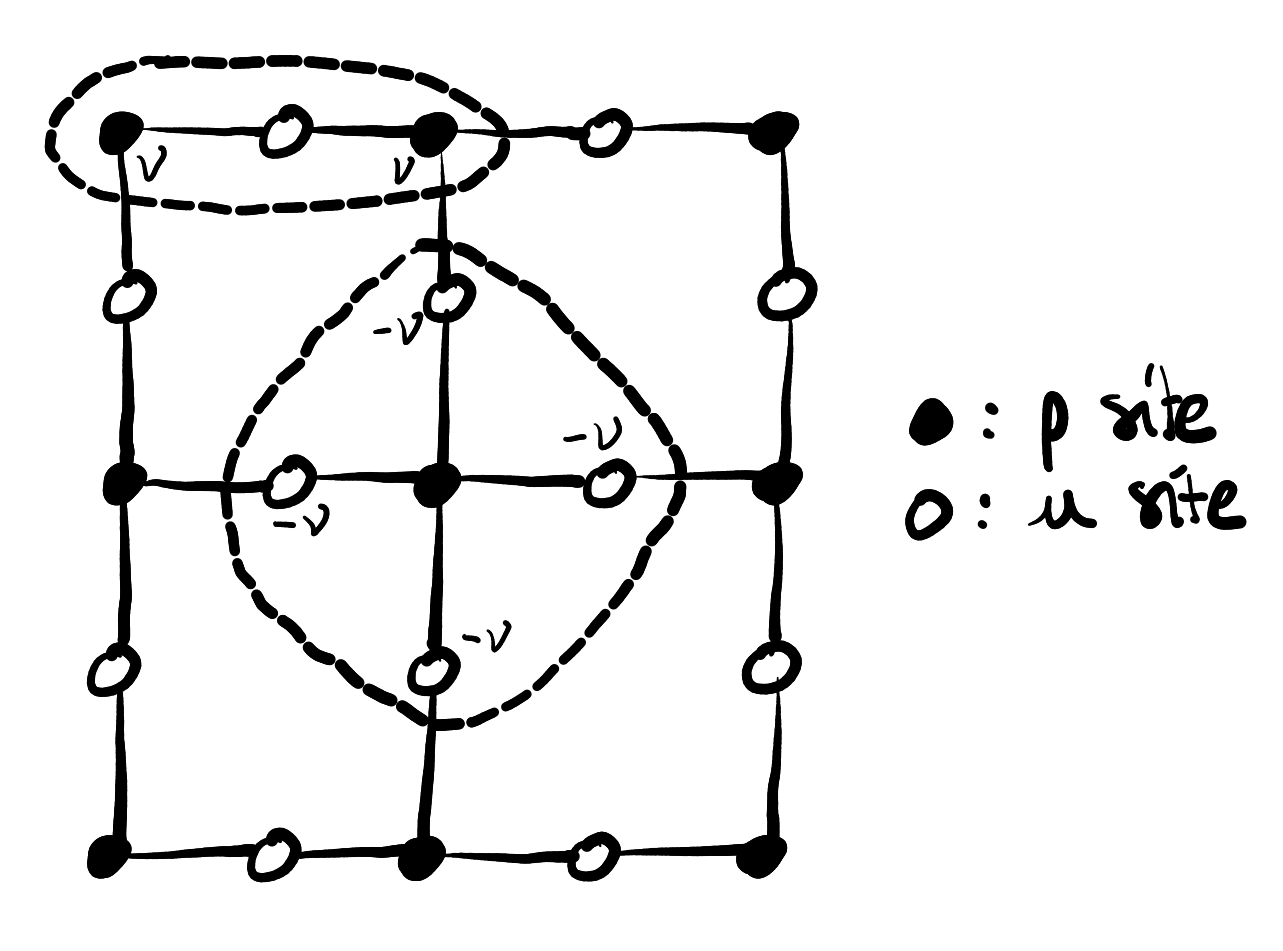
\includegraphics[scale=0.2]{graphs/hypercubic.png}
            \caption{Hypercubic lattice in $d=2$.}
            \label{fig:hypercubic}
        \end{figure}
        
        Now introduce the fermionic operators corresponding to the single-\electron states around $p$ and $u$ as 
        \be a_{p\sigma} = c_{p\sigma} - \nu \sum_{u \text{ n.n. to } p}c_{u\sigma} \qq{and} b_{u\sigma} = c_{u\sigma} + \nu \sum_{p \text{ n.n. to } u}c_{p\sigma} \ee
        Then write the Hamiltonian as
        \be \mc H = \mc H_\text{hop} + \mc H_\text{int} = t \sum_{u,\sigma} b^\dagger_{u\sigma} b_{u\sigma} + U\sum_j n_{j\uparrow} n_{j\downarrow} \label{eq:tasaki_hubbard} \ee
        With this particular form, the hopping term interestingly exhibits the same structure as the 3-site toy model for $d=1$, since hopping between all n.n. is possible as well as between $p$ sites separated by distance 1. From this, Tasaki's flat-band ferromagnetism follows.
        
        Consider the Hubbard model given in \eqref{eq:tasaki_hubbard} with $N=L^d$ \electron, $t, \nu, U>0$. Then the ground states have $S_\text{tot} = \frac{N}{2}$ and are unique apart from the $(2S_\text{tot}+1)$-fold degeneracy.
        
        One is not proving this theorem but shall construct the ground states of this system when half-filled --- remember that $u$ sites do not contribute with any \electron. From the orthogonality between $u$- and $p$-single-\electron states, one finds $\{ b_{u\sigma},a^\dagger_{p\sigma} \}=0$ --- since $\{c_\sigma(\psi),c^\dagger_{\sigma'}(\psi')\}=\braket{\psi}{\psi'} \delta_{\sigma \sigma'}$ --- which implies $[ b^\dagger_{u\sigma}b_{u\sigma},a^\dagger_{p\sigma}]=0$. One encourages the reader to check these relations. Therefore
        \be \mc H |\psi_\alpha ^\uparrow\rangle = 0 \qq{with} |psi_\alpha ^\uparrow\rangle = \left[\prod_p a^\dagger_{p\uparrow}\right] \ket 0 \ee
        since $\mc H_\text{hop}$ is a sum of $b^\dagger_{u\sigma}b_{u\sigma}$ and $\mc H_\text{int}$ counts the number of doubly-occupied sites which do not exist when everyone has the same spin. Thus $|\psi_\alpha ^\uparrow\rangle$ is ferromagnetic state of energy $0$. This allows to write the ground states as
        \be | \psi_\text{GS}^{(M)}\rangle = (S^-_\text{tot})^{\frac{N}{2}-M} |\psi_\alpha ^\uparrow\rangle \qq{with} M=-N/2, -N/2+1,\dotsc, N/2 \ee
        
        Now, remains to find the band structure and observe that the system indeed exhibits flat-band ferromagnetism. Start by rewriting the Hamiltonian \eqref{eq:tasaki_hubbard} with
        \be \mc H_\text{hop} = \sum_{i,j,\sigma} t_{ij} c^\dagger_{i\sigma}c_{j\sigma} \qq{with} t_{ij} = \begin{cases} \nu t & \text{if } i,j \text{ n.n.} \\ \nu^2 t & \text{if } i,j \text{ s.n. } p \text{ sites} \\ t & \text{if } i=j=u \\ 2d\nu^2 t & \text{if } i=j=p \\ 0 & \text{otherwise} \end{cases} \ee
        Then solve the for the single-\electron SE to have the band structure
        \be \varepsilon_\mu (k) = \begin{cases} 0 & \mu = 1 \\ t & \mu = 2,\dotsc, d \\ t + 2\nu^2 t\sum_{j=1}^d (1 + \cos k_j) & \mu = d+1 \end{cases} \ee
        which is straightforward to derive \emph{eg} in $d=2$ as
        \be \mc H = \pmqty{2\nu^2 t\sum_{j=x,y} (1 + \cos k_j) & \nu t (1+e^{-ik_x}) & \nu t (1+e^{-ik_y}) \\ \nu t (1+e^{ik_x}) & t & 0 \\ \nu t (1+e^{ik_y}) & 0 & t} \ee
        which generates the band structure
        \be 0 = \varepsilon(t-\varepsilon)\left[ \varepsilon - t - 2\nu^2 t\sum_{j=x,y} (1 + \cos k_j) \right] \ee
        having used the identity $\abs{\nu t (1+e^{ik_j})}^2 = 2 \nu^2 t^2(1 + \cos k_j)$. Therefore $d$ bands are flat, the lowest one being non-degenerate with energy $0$ and the other $d-1$ are degenerate with energy $t$. Thus take the lowest one, which is more interesting since it has $L^d$ states separated from the others by a gap $t>0$. Hence, for the many \electron problem without interaction $U=0$ the zero-energy ground states are 
        \be \left[\prod_{p\in \{\uparrow\}} a^\dagger_{p\uparrow}\right]  \left[\prod_{p\in \{\downarrow\}} a^\dagger_{p\downarrow}\right] \ket 0 \ee
        and thereby have spin $S_\text{tot} = 0, \frac{1}{2},\dotsc, \frac{N}{2}$ $\rightarrow$ paramagnetism. But introducing $U>0$ lifts the degeneracy to select the full ferromagnetic ground state with highest $S_\text{tot} = \frac{N}{2}$ to be the only ground state, according to Tasaki's theorem aforementioned.
        
        Finally, it is possible and interesting to relate this to the 3-site toy model since models exhibiting flat-band ferromagnetism are 3-site toy models assemblies !
        